% Sept-13 overview -- QA for VeriContest, the ProofGen dataset landscape, CUDA+Verus
% UIUC SRSE 2026, September 13, 2026
% Build: pdflatex 2026-09-13-overview.tex  (run twice)

\documentclass[aspectratio=169,10pt]{beamer}

\usepackage[T1]{fontenc}
\usepackage[utf8]{inputenc}
\usepackage[sfdefault]{FiraSans}
\usepackage[scaled=0.85]{FiraMono}
\usepackage{listings}
\usepackage{tikz}
\usepackage{tcolorbox}
\usepackage{booktabs}
\usepackage{graphicx}
\graphicspath{{../img/}}

\usetheme{metropolis}
\metroset{sectionpage=progressbar, numbering=fraction, progressbar=frametitle}

\usetikzlibrary{arrows.meta, positioning, calc, fit, backgrounds}
\tcbuselibrary{skins}

% Palette
\definecolor{lgInk}{HTML}{23373B}
\definecolor{lgAccent}{HTML}{C25E00}
\definecolor{lgTeal}{HTML}{0F7B8A}
\definecolor{lgRed}{HTML}{B3282D}
\definecolor{lgGreen}{HTML}{2E7D32}
\definecolor{lgGrey}{HTML}{6B7A7D}
\definecolor{lgWash}{HTML}{F2F4F4}
\definecolor{lgWashWarm}{HTML}{FBF1E6}

\setbeamercolor{normal text}{fg=lgInk}
\setbeamercolor{frametitle}{bg=lgInk, fg=white}
\setbeamercolor{progress bar}{fg=lgAccent}
\setbeamercolor{alerted text}{fg=lgAccent}

% Code listings
\lstdefinestyle{verus}{
  basicstyle=\ttfamily\scriptsize\color{lgInk},
  keywordstyle=\color{lgTeal}\bfseries,
  morekeywords={ensures,requires,invariant,decreases,proof,assert,spec,fn,let,ghost,loop,while,if,else,use,pub,result},
  showstringspaces=false,
  breaklines=false,
  columns=fullflexible,
  keepspaces=true,
  aboveskip=1pt, belowskip=1pt,
}
\lstset{style=verus}

% Inline helpers
\newcommand{\code}[1]{{\ttfamily #1}}
\newcommand{\hd}[1]{\textbf{\color{lgTeal}#1}}
\newcommand{\good}[1]{{\color{lgGreen}#1}}
\newcommand{\bad}[1]{{\color{lgRed}#1}}

% Boxes
\newtcolorbox{callout}[1][lgAccent]{
  enhanced, colback=lgWashWarm, colframe=#1,
  boxrule=0.1pt, leftrule=2.5pt, arc=1.5pt,
  left=6pt, right=6pt, top=4pt, bottom=4pt, boxsep=0pt,
}

\newtcolorbox{codebox}[2][lgGrey]{
  enhanced, colback=lgWash, colframe=#1,
  boxrule=0.1pt, leftrule=2.5pt, arc=1.5pt,
  left=6pt, right=4pt, top=3pt, bottom=3pt, boxsep=0pt,
  title={\scriptsize\bfseries\color{#1}#2},
  fonttitle=\bfseries, coltitle=#1,
  colbacktitle=lgWash, titlerule=0pt,
  attach title to upper={\par\vspace{1pt}},
}

% Formal definition box
\newtcolorbox{defbox}[1]{
  enhanced, colback=white, colframe=lgInk,
  boxrule=0.7pt, arc=1.5pt,
  left=6pt, right=6pt, top=4pt, bottom=4pt, boxsep=0pt,
  title={\scriptsize\bfseries #1}, fonttitle=\bfseries,
  colbacktitle=lgInk, coltitle=white,
}

% TikZ styles
\tikzset{
  stage/.style={
    draw=lgInk, line width=0.7pt, rounded corners=2pt,
    fill=white, inner sep=5pt, align=center,
    font=\scriptsize, text=lgInk, minimum height=9mm
  },
  gate/.style={stage, draw=lgRed, fill=lgRed!8, text=lgRed, font=\scriptsize\bfseries},
  okstage/.style={stage, draw=lgGreen, fill=lgGreen!8, text=lgGreen},
  mem/.style={stage, draw=lgTeal, fill=lgTeal!8, text=lgTeal},
  flow/.style={-{Stealth[length=2mm]}, line width=0.7pt, draw=lgInk},
  flowr/.style={-{Stealth[length=2mm]}, line width=0.9pt, draw=lgRed},
  flowt/.style={-{Stealth[length=2mm]}, line width=0.7pt, draw=lgTeal},
  lbl/.style={font=\tiny\itshape, text=lgGrey, inner sep=2pt},
}

% Title
\title{Three Threads}
\subtitle{QA on the VeriContest dataset $\cdot$ ProofGen bottlenecks across the literature $\cdot$ NVIDIA CUDA on Rust}
\date{September 13, 2026}
\institute{UIUC SRSE 2026 $\cdot$ Mahadi}

\begin{document}

\maketitle

% =====================================================================
\section{QA on the VeriContest dataset}

% SECTION 1 -- slide 1: lynette rejects ground truth, measured on two suites.
\begin{frame}{lynette rejects ground truth, on both suites}

{\scriptsize
Last time: \code{lynette compare} rejects VeriContest's own reference proofs. Since then the same
sweep has been run against a second benchmark, and the VeriContest corpus has been pinned and
vendored so the number can be re-derived.
}

\vspace{6pt}
\begin{center}
{\scriptsize
\begin{tabular}{llrrl}
\toprule
\textbf{suite} & \textbf{pair compared} & \textbf{n} & \textbf{rejected} & \textbf{build $\cdot$ corpus} \\
\midrule
Verus-Bench & \code{unverified.rs} vs \code{verified.rs}  & 149 & \bad{\textbf{84}} \ (56.4\%)
  & \code{2f9aff36} $\cdot$ \code{compare -t} \\
VeriContest & \code{code\_spec.rs} vs \code{verified.rs}  & 946 & \bad{\textbf{298}} \ (31.5\%)
  & \code{fd9edd2f0} $\cdot$ \code{compare -t} \\
            &                                             &     & \bad{\textbf{371}} \ (39.2\%)
  & \quad{} \code{-t --spec}, \code{benchmark@0cc50f5} \\
\bottomrule
\end{tabular}
}
\end{center}

\vspace{6pt}
\begin{columns}[T]
\begin{column}{0.48\textwidth}
{\scriptsize
\hd{These are the benchmarks' own answers}\\
Every problem ships a reference proof that is, by construction, a correct answer to the task it
poses. Nothing held to lynette could have produced the rejected ones.

\vspace{4pt}
{\color{lgGrey}A further \textbf{7} VeriContest problems lynette cannot parse at all. They are
counted separately: \code{compare} exits 1 for a parse failure and for a difference alike, so
calling them rejections would report a verdict lynette never reached. Verus accepts all seven.}
}
\end{column}

\begin{column}{0.48\textwidth}
\begin{callout}[lgAccent]
\scriptsize
\textbf{The pipeline runs \code{-t} alone}, which never sets \code{spec}, so every
\code{spec fn} is erased from both sides and no spec-function body is ever compared. Turning
\code{--spec} on adds \textbf{73} rejections and loses none.
\end{callout}

\vspace{5pt}
{\scriptsize\color{lgGrey}A rejection here is counted, not interpreted: which of the 371 are the
lynette's fault is a separate exercise, and is not what this section claims.}
\end{column}
\end{columns}

\end{frame}

% =====================================================================
% SECTION 1 -- slide 2: the concrete case first, then why, then the fix.
\begin{frame}[fragile]{cf1200C: the whole objection is one import}

{\scriptsize
A VeriContest reference proof, the benchmark's own answer, rejected by lynette. Deghosted,
this is its \emph{entire} difference from \code{code\_spec.rs}:
}

\vspace{4pt}
\begin{center}
\begin{minipage}{0.58\linewidth}
\begin{codebox}[lgRed]{\code{verified.rs} vs \code{code\_spec.rs}, after erasure}
{\ttfamily\scriptsize
\phantom{+ }use vstd::prelude::*;\\
{\color{lgGreen}+ }use vstd::arithmetic::div\_mod::*;
}
\end{codebox}
\end{minipage}
\end{center}

\vspace{3pt}
{\scriptsize
It exists solely to name three lemmas, all called \emph{only} from \code{proof fn} bodies.
Everything else erases cleanly and matches. lynette exits 1; Verus never runs.
}

\vspace{5pt}
{\scriptsize
\hd{Why.}\ Verus separates \textbf{ghost} code, everything that exists only for the
proof, from the program itself. An import written at the top of the file is not ghost code: it
is ordinary module-level Rust, so lynette compares it like any other program text. The lemmas it
names \emph{are} ghost, and erase; the line that imports them does not.
}

\vspace{4pt}
\begin{callout}[lgGreen]
\scriptsize
\textbf{The recommended form.} Write the \code{use} \emph{inside} the \code{proof fn} or
\code{proof \{\}} that needs it, or fully qualify the call sites. lynette accepts; Verus still
verifies.
\end{callout}

\end{frame}

% =====================================================================
% SECTION 1 -- slide 3: the proposal.
\begin{frame}{Proposal: an advisory check on the dataset itself}

{\scriptsize
Nothing here asks the authors to change how ProofGen is scored. It asks that a problem not enter
the benchmark carrying an annotation lynette will object to: checked when the problem is
written, not when a model is graded.
}

\vspace{6pt}
\begin{center}
\resizebox{0.88\linewidth}{!}{%
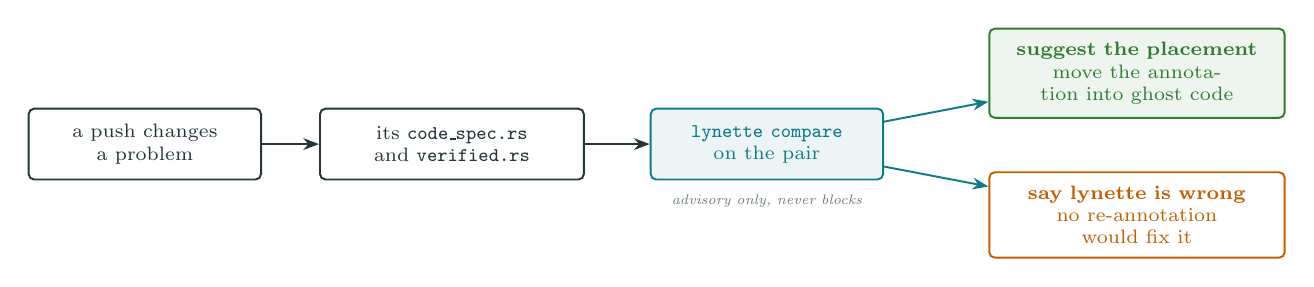
\begin{tikzpicture}[node distance=7mm]
  \node[stage, text width=26mm] (push) at (0,0) {a push changes\\a problem};
  \node[stage, text width=30mm] (pair) at (3.9,0) {its \code{code\_spec.rs}\\and \code{verified.rs}};
  \node[mem,   text width=26mm] (lyn)  at (7.9,0) {\code{lynette compare}\\on the pair};
  \node[okstage, text width=34mm] (fix) at (12.6,0.9) {\textbf{suggest the placement}\\
    move the annotation into ghost code};
  \node[stage, draw=lgAccent, text=lgAccent, text width=34mm] (wrong) at (12.6,-0.9)
    {\textbf{say lynette is wrong}\\no re-annotation would fix it};

  \draw[flow]  (push) -- (pair);
  \draw[flow]  (pair) -- (lyn);
  \draw[flowt] (lyn) -- (fix);
  \draw[flowt] (lyn) -- (wrong);
  \node[lbl, below=1mm of lyn, text width=30mm, align=center] {advisory only, never blocks};
\end{tikzpicture}%
}
\end{center}

\vspace{4pt}
\begin{columns}[T]
\begin{column}{0.47\textwidth}
{\scriptsize
\hd{Why it belongs upstream}\\
The benchmark's own consistency checker \textbf{strips \code{use} items before comparing}, so an
import difference is invisible at authoring time and surfaces only later, as a model's
\code{unsafe\_code\_or\_spec\_change}. The check is proposed as a PR to VeriContest.
}
\end{column}

\begin{column}{0.49\textwidth}
{\scriptsize
\hd{Why it has to say when lynette is wrong}\\
Not every rejection has a fix. Where the erasure itself manufactured the difference, there is no
placement that satisfies lynette, and an advisory that only ever suggests re-annotation would send
an author looking for one.
}
\end{column}
\end{columns}

\end{frame}

% =====================================================================
\section{ProofGen bottlenecks across the literature}

% =====================================================================
% SECTION 2 -- slide 0: what the ProofGen task is.
\begin{frame}{What every one of these papers is doing}

{\scriptsize
One task, shared across the whole literature: \textbf{spec $+$ code $\rightarrow$ proof}. The
model is handed a program together with its specification and no proof, and must supply the
annotations that make Verus accept it.
}

\vspace{8pt}
\begin{center}
\resizebox{0.92\linewidth}{!}{%

\begin{tikzpicture}[node distance=8mm]
  \node[stage, text width=34mm] (in) at (0,0)
    {\textbf{one task}\\program $+$ contract,\\proof annotations stripped};
  \node[mem, text width=26mm] (sys) at (4.8,0) {the system\\under study};
  \node[stage, text width=30mm] (out) at (9.0,0)
    {the same program,\\proof added};
  \node[okstage, text width=22mm] (ver) at (13.0,0) {\textbf{Verus}\\verified?};

  \draw[flow] (in) -- (sys);
  \draw[flow] (sys) -- (out);
  \draw[flow] (out) -- (ver);
  \node[lbl, below=6mm of sys, text width=150mm, align=center]
    {adds invariants, asserts and lemmas; the program and the contract may not change};
\end{tikzpicture}%
}
\end{center}

\vspace{8pt}
\begin{columns}[T]
\begin{column}{0.47\textwidth}
{\scriptsize
\hd{What a benchmark is}\\
A fixed set of such tasks, each shipping a reference proof written by a human. The reported
number is the fraction of the set that Verus accepts.
}
\end{column}

\begin{column}{0.49\textwidth}
{\scriptsize
\hd{Why the tasks are the variable}\\
The mechanism differs from paper to paper: prompting, retrieval, tree search, counterexamples,
agents. The task never does. So a result is a claim about a system \emph{and} about the set of
tasks it was run on.
}
\end{column}
\end{columns}

\end{frame}

% =====================================================================
% SECTION 2 -- slide 2: the full survey, every paper against every suite it uses.
\begin{frame}{Every paper, every suite it reports on}

{\scriptsize
{\color{lgGrey}Each number is that paper's own, under its own model and Verus version; every
system here generates and then repairs, so these are end-to-end task success rates.}
\ \hd{Bold} = built from real systems code.
}

\vspace{3pt}
\begin{center}
{\tiny
\renewcommand{\arraystretch}{0.88}
\setlength{\tabcolsep}{4pt}
\begin{tabular}{@{}llrrl@{}}
\toprule
\textbf{paper} & \textbf{benchmark} & \textbf{n} & \textbf{solved} & \textbf{kind} \\
\midrule
Yao et al.\ '23 & Diffy-derived vector programs & 20 & 38/55 seg & textbook, human in loop \\
\addlinespace[2pt]
AlphaVerus '24  & MBPP                    & --    & 65.7\% & textbook \\
                & HumanEval               & --    & 32.9\% & textbook \\
\addlinespace[2pt]
AutoVerus '25   & Verus-Bench             & 150   & \good{91.3\%} & textbook + Diffy \\
\addlinespace[2pt]
SAFE '25        & VerusBench              & 139   & 52.5\% & textbook \\
                & CodeNet-Test            & 1,435 & 48.5\% & synthesised \\
\addlinespace[2pt]
RagVerus '25    & VerusBench              & 139   & 60.4\% & textbook \\
                & \textbf{RepoVBench}     & 383   & 19.6\% & \textbf{VeriSMo, confidential VM} \\
\addlinespace[2pt]
VeruSAGE '25    & \textbf{VeruSAGE-Bench} & 849   & 81\%   & \textbf{8 verified systems} \\
\addlinespace[2pt]
ExVerus '26     & VerusBench              & 146   & 88.4\% & textbook + Diffy \\
                & Dafny2Verus             & 67    & \good{95.5\%} & textbook \\
                & HumanEval-Verus         & 68    & 41.2\% & textbook \\
                & LCBench                 & 28    & 28.6\% & LeetCode, $\sim$200 LoC \\
                & ObfsBench               & 266   & $>$73\% & obfuscated VerusBench \\
                & InvariantInjectBench    & 187   & --     & \emph{repair only}: seeded bad invariant \\
\addlinespace[2pt]
KVerus '26      & Verus-Bench             & 150   & 88\%   & textbook + Diffy \\
                & MBPP                    & 78    & 83\%   & textbook \\
                & Human-Eval              & 85    & 64\%   & textbook \\
                & MathSpec-Bench          & --    & 77.9\% & Lean 4 maths, repo \\
                & \textbf{Memory Allocator} & --  & 56.2\% & \textbf{allocator, repo} \\
                & \textbf{CortenMM}       & --    & 31.3\% & \textbf{Asterinas kernel MM} \\
\addlinespace[2pt]
VeriContest '26 & VeriContest             & 946   & \bad{13.95\%} & LeetCode + Codeforces \\
\bottomrule
\end{tabular}
}
\end{center}

\end{frame}

% =====================================================================
% SECTION 2 -- slide 1: a mechanism is only visible on a hard enough dataset.
\begin{frame}{A mechanism only shows its strength on a hard enough dataset}

{\scriptsize
One paper, one model, one harness, four datasets, so the only thing varying is the difficulty
of the tasks. The better mechanism wins by more and more as the dataset gets harder, and by
nothing at all once the dataset is saturated.
}

\vspace{6pt}
\begin{center}
{\scriptsize
\hd{ExVerus vs AutoVerus, Sonnet-4.5}\quad{\color{lgGrey}success rate, \%}\\[5pt]
\begin{tabular}{lrrr}
\toprule
\textbf{dataset} & \textbf{n} & \textbf{AutoVerus} & \textbf{ExVerus} \\
\midrule
Dafny2Verus      & 67  & 95.5 & \good{95.5} \\
VerusBench       & 146 & 75.3 & 88.4 \\
HumanEval-Verus  & 68  & 27.9 & 41.2 \\
LCBench          & 28  & \bad{14.3} & \bad{28.6} \\
\bottomrule
\end{tabular}
}
\end{center}

\vspace{6pt}
\begin{columns}[T]
\begin{column}{0.47\textwidth}
\begin{callout}[lgGrey]
\scriptsize
\textbf{On a saturated dataset the mechanism is invisible.} Dafny2Verus is already at 95.5 for
both, so no technique can show anything there.
\end{callout}
\end{column}

\begin{column}{0.49\textwidth}
\begin{callout}[lgAccent]
\scriptsize
\textbf{The harder the tasks, the more the mechanism is worth.} On LCBench ExVerus
\textbf{doubles} AutoVerus. Progress is only measurable where there is room to measure it.
\end{callout}
\end{column}
\end{columns}

\end{frame}

% =====================================================================
% SECTION 2 -- slide 3: taxonomy of problem kinds, and the conclusion.
\begin{frame}{A dissection of the kinds of problems current datasets provide}

\vspace{2pt}
\begin{center}
{\tiny
\renewcommand{\arraystretch}{1.15}
\setlength{\tabcolsep}{5pt}
\begin{tabular}{@{}p{27mm}p{38mm}p{16mm}p{52mm}@{}}
\toprule
\textbf{kind of problem} & \textbf{suites} & \textbf{tasks} & \textbf{what one task looks like} \\
\midrule
competitive programming
  & VeriContest $\cdot$ CodeNet-Test $\cdot$ LCBench
  & 946 $\cdot$ 1,435 $\cdot$ 28
  & one function, a loop over an array, an interview or contest algorithm \\
entry-level / textbook
  & MBPP $\cdot$ HumanEval-Verus $\cdot$ CloverBench $\cdot$ Dafny2Verus
  & 78 $\cdot$ 68 $\cdot$ 11 $\cdot$ 67
  & string and list operations, sorting, searching, array transforms \\
invariant-stress arrays
  & Diffy
  & 38
  & accumulator loops with deliberately awkward inductive relationships \\
perturbations of the above
  & ObfsBench $\cdot$ InvariantInjectBench
  & 266 $\cdot$ 187
  & the same problems, obfuscated, or seeded with one bad invariant \\
\midrule
\textbf{real systems code}
  & \textbf{VeruSAGE-Bench} $\cdot$ \textbf{RepoVBench} $\cdot$ \textbf{KVerus repo-level}
  & \textbf{849} $\cdot$ \textbf{383} $\cdot$ \textbf{359}
  & \textbf{OS kernels, allocators, page tables, a confidential-VM security module,
    a binary parser} \\
\bottomrule
\end{tabular}
}
\end{center}

\vspace{5pt}
\begin{columns}[T]
\begin{column}{0.45\textwidth}
{\scriptsize
\hd{The two are not the same exercise}\\[2pt]
\begin{tabular}{lrr}
\toprule
 & \textbf{Verus-Bench} & \textbf{VeruSAGE-Bench} \\
\midrule
LoC per task     & 32   & \textbf{$\sim$947} \\
lemmas per task  & 0.07 & \textbf{2.4} \\
\bottomrule
\end{tabular}
}
\end{column}

\begin{column}{0.51\textwidth}
\begin{callout}[lgAccent]
\scriptsize
Only \textbf{three} suites are built from systems code, and only one of them is substantial.
A mechanism is only visible on hard tasks, and the field has very few. \textbf{What the
literature lacks is relevant datasets, more than it lacks proof techniques.}
\end{callout}
\end{column}
\end{columns}

\end{frame}

% =====================================================================
% SECTION 2 -- slide 4: the honest answer, and the bridge to section 3.
\begin{frame}{So Mahadi, can you improve ProofGen or not?}

\begin{columns}[T]
\begin{column}{0.48\textwidth}
{\scriptsize
\hd{What I set out to do}\\
Agentic-loop mechanisms, aimed at VeriContest, to beat \textbf{13.95\%}.

\vspace{5pt}
\hd{What reading the papers did to that}\\
The draft ideas are already in the literature, and implemented better than I had them:
ExVerus's counterexample-guided repair and RagVerus's retrieval both go further than what I had
drawn up.

\vspace{5pt}
\hd{Can I still do better on current datasets?}\\
\textbf{About 70\% confident yes}, and \emph{how} is a different talk from this one.
}
\end{column}

\begin{column}{0.48\textwidth}
{\scriptsize
\hd{But then what would the result mean?}\\
Suppose I add technique, beat a current number by a margin, and run the same thing on
VeriContest. Against what do I claim the win?
}

\vspace{5pt}
\begin{center}
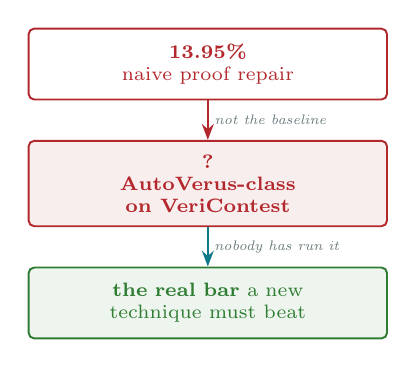
\begin{tikzpicture}[node distance=4mm]
  \node[stage, draw=lgRed, text=lgRed, text width=42mm] (a)
    {\textbf{13.95\%}\\naive proof repair};
  \node[gate, text width=42mm, below=5mm of a] (b)
    {\textbf{?}\\AutoVerus-class on VeriContest};
  \node[okstage, text width=42mm, below=5mm of b] (c)
    {\textbf{the real bar} a new technique must beat};
  \draw[flowr] (a) -- (b) node[lbl, midway, right] {not the baseline};
  \draw[flowt] (b) -- (c) node[lbl, midway, right] {nobody has run it};
\end{tikzpicture}
\end{center}
\end{column}
\end{columns}

\vspace{6pt}
\begin{callout}[lgAccent]
\scriptsize
\textbf{13.95\% is not the number to beat}: it is what a naive proof-repair loop scores. The
honest comparison is to run the established mechanisms on VeriContest first, find out what \emph{they} score, and beat that.
\ \hd{And if ProofGen is hard to improve substantially, what then?} That is the next section.
\end{callout}

\end{frame}

% =====================================================================
\section{NVIDIA CUDA on Rust}

% =====================================================================
% SECTION 3 -- slide 1: the proposal, and the questions the section asks.
\begin{frame}{Contribute a benchmark dataset for LLM-written CUDA kernels in Rust}

\begin{columns}[T]
\begin{column}{0.52\textwidth}
{\scriptsize
\hd{Section 2's conclusion, applied}\\[2pt]
Rust exists to write \textbf{low-level systems} safely. The ProofGen literature barely evaluates
on that kind of code: three suites, one of them substantial.

\vspace{5pt}
And GPU kernels are certainly not among them. They \emph{could not} be: NVIDIA brought CUDA to
Rust on \textbf{8 September 2026}, five days ago.

\vspace{6pt}
\hd{So what I am doing}\\[2pt]
A \textbf{feasibility study} of whether formal verification is needed here at all, started from
knowing nothing about GPU kernels.
}
\end{column}

\begin{column}{0.44\textwidth}
\begin{callout}[lgGrey]
\scriptsize
Academia runs on \emph{publish or perish}. As a Fall '27 applicant with no publication, mine for
the next 60 days is \textbf{submit or perish}, which is why a new benchmark dataset is the bet
I think is worth making.
\end{callout}

\vspace{6pt}
{\scriptsize
\hd{Why a dataset rather than a technique}\\
Section 2: a technique has to beat an established number on an established suite. A dataset that
does not exist yet has no incumbent to displace.
}
\end{column}
\end{columns}

\vspace{7pt}
\begin{defbox}{What this section asks}
\scriptsize
\textbf{1.}\ Is there scope, or need, for \textbf{functional correctness} of CUDA kernels at
all? \\[2pt]
\textbf{2.}\ Does that change when the kernel is written in \textbf{Rust}? \\[2pt]
\textbf{3.}\ Can \textbf{Verus} handle it? \\[2pt]
\textbf{4.}\ If it can, where would adding \code{requires} / \code{ensures} actually be
interesting?
\end{defbox}

\end{frame}

% =====================================================================
% SECTION 3 -- slide 2: what ProofWright does, and what it says about Verus.
\begin{frame}{ProofWright: agentic formal verification of CUDA}

{\scriptsize
arXiv 2511.12294, November 2025. Formal verification of \textbf{LLM-generated CUDA kernels},
because runtime testing has limited coverage and is \emph{``vulnerable to reward hacking.''}
}

\vspace{6pt}
\begin{columns}[T]
\begin{column}{0.5\textwidth}
{\scriptsize
\hd{What it does}\\[2pt]
\textbf{VerCors Agent} synthesises deductive annotations from a knowledge base, an annotation
guide and an error-fix database, giving SMT-backed \textbf{memory safety and data-race freedom}.

\vspace{3pt}
\textbf{Rocq Agent} extracts the computational specification from the PyTorch source and
proves \textbf{semantic equivalence} against the generated CUDA, on \code{MLRocq}, a verified
library of tensor operators.

\vspace{5pt}
\hd{On KernelBench L1}\ {\color{lgGrey}100 problems, Claude-4-Sonnet}\\[3pt]
\begin{tabular}{lr}
\toprule
\good{verified}: memory \& thread safety & \good{\textbf{74\%}} \\
SMT solver instability & 17\% \\
agent failure & 9\% \\
\bottomrule
\end{tabular}\ \ {\color{lgGrey}$\sim$3 min/kernel}
}
\end{column}

\begin{column}{0.46\textwidth}
{\scriptsize
\hd{What its authors say about Verus}\\[2pt]
They compare themselves directly to AutoVerus, and make three claims.
}

\vspace{4pt}
\begin{callout}[lgTeal]
\scriptsize
\textbf{1.}\ Verus, \emph{like VerCors}, ``suffers from low amounts of training data.''

\vspace{3pt}
\textbf{2.}\ Verus programs get Rust's type-system guarantees, so they \textbf{need not prove
memory safety or data-race freedom} for safe Rust, less burden on the LLM to reason about
concurrency or memory safety.

\vspace{3pt}
\textbf{3.}\ AutoVerus \emph{assumes} the specification is already given in Verus; ProofWright
extracts the functional specification from a high-level implementation.
\end{callout}
\end{column}
\end{columns}

\end{frame}

% =====================================================================
% SECTION 3 -- slide 3: CUDA-on-Rust collapses ProofWright's pipeline.
\begin{frame}{CUDA on Rust collapses that pipeline}

{\scriptsize
ProofWright's architecture is \emph{forced} by CUDA being C++: the specification lives in
PyTorch, the proof lives in Rocq, the kernel lives in CUDA: three languages, two verifiers, and
an \emph{untrusted lowering stage} between them, which the paper itself flags.
}

\vspace{6pt}
\begin{center}
\resizebox{0.96\linewidth}{!}{%
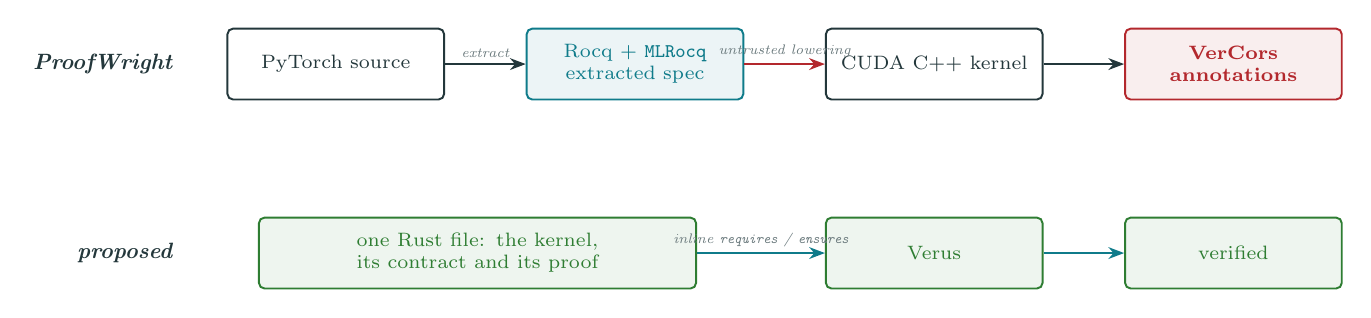
\begin{tikzpicture}
  % ProofWright row
  \node[lbl, text=lgInk, anchor=east] at (-0.4,1.2) {\footnotesize\bfseries ProofWright};
  \node[stage, text width=24mm] (py)  at (1.6,1.2) {PyTorch source};
  \node[mem,   text width=24mm] (rocq)at (5.4,1.2) {Rocq $+$ \code{MLRocq}\\extracted spec};
  \node[stage, text width=24mm] (cu)  at (9.2,1.2) {CUDA C++ kernel};
  \node[gate,  text width=24mm] (vc)  at (13.0,1.2) {VerCors\\annotations};
  \draw[flow]  (py) -- (rocq) node[lbl, midway, above] {extract};
  \draw[flowr] (rocq) -- (cu) node[lbl, midway, above] {untrusted lowering};
  \draw[flow]  (cu) -- (vc);

  % Proposed row
  \node[lbl, text=lgInk, anchor=east] at (-0.4,-1.2) {\footnotesize\bfseries proposed};
  \node[okstage, text width=52mm] (rs) at (3.4,-1.2)
    {one Rust file: the kernel, its contract and its proof};
  \node[okstage, text width=24mm] (vs) at (9.2,-1.2) {Verus};
  \node[okstage, text width=24mm] (ok) at (13.0,-1.2) {verified};
  \draw[flowt] (rs) -- (vs) node[lbl, midway, above] {inline \code{requires} / \code{ensures}};
  \draw[flowt] (vs) -- (ok);
\end{tikzpicture}%
}
\end{center}

\vspace{6pt}
\begin{columns}[T]
\begin{column}{0.47\textwidth}
\begin{callout}[lgGreen]
\scriptsize
\textbf{What collapsing it buys.} No specification to extract from a high-level framework. No
second, interactive theorem prover. No lowering gap between the thing proved and the thing that
runs.
\end{callout}
\end{column}

\begin{column}{0.49\textwidth}
\begin{callout}[lgAccent]
\scriptsize
\textbf{And by their own argument, the easy half is already done.} Safe Rust gives memory safety
and data-race freedom for free, so the work moves to exactly where ProofWright got least far:
\textbf{functional correctness}.
\end{callout}
\end{column}
\end{columns}

\end{frame}

% =====================================================================
% SECTION 3 -- slide 4: feasibility intuition from VeriSMo, mapped onto a kernel.
\begin{frame}{Have I checked a real codebase?}

\vspace{4pt}
\begin{columns}[T]
\begin{column}{0.36\textwidth}
{\scriptsize
\hd{Verus is already in industry}\\[2pt]
Microsoft, Amazon. \textbf{VeriSMo} and \textbf{Anvil}: two of three OSDI'24 best papers.
\textbf{CortenMM}: concurrent memory management.

\vspace{6pt}
\hd{The intuition}\\[2pt]
VeriSMo's 869 \code{requires} sit at \textbf{trust boundaries}, not everywhere. \code{external\_body}
means: \emph{body unverified, contract enforced}.

\vspace{4pt}
Verification is not proving everything. It is \textbf{bounding what you trust}.
}
\end{column}

\begin{column}{0.6\textwidth}
{\scriptsize
\hd{The same placement, on a cuTile MoE kernel}\\[3pt]
{\tiny
\renewcommand{\arraystretch}{1.25}
\begin{tabular}{@{}p{20mm}p{15mm}p{33mm}@{}}
\toprule
\textbf{where} & \textbf{contract} & \textbf{what it buys} \\
\midrule
descriptor loaders & \code{requires} & five unchecked \code{assume} axioms become caller
  obligations \\
kernel entry & \code{requires} & restores the shape agreement the code computes, then discards \\
scheduler loop & \code{invariant} & div-by-zero on an empty expert; the tile partition \\
\code{mma}, pointer \& tensor-view primitives & \code{external\_body} $+$ contract & bounds the
  trusted base; float semantics stay \emph{below} it \\
\bottomrule
\end{tabular}
}
}

\vspace{5pt}
\begin{callout}[lgAccent]
\scriptsize
GPU kernels already mark their trust boundaries, with \code{unsafe} and with \code{assume}.
\end{callout}
\end{column}
\end{columns}

\end{frame}

% =====================================================================
% SECTION 3 -- slide 5: real cutile-rs code, and the contract it is missing.
\begin{frame}[fragile]{The contracts are already written, as \code{assume}, not \code{requires}}

{\scriptsize
\href{https://github.com/NVlabs/cutile-rs/blob/2eed75e8f552be31216ddf2019288f03dfec4939/cutile-kernels/src/experimental/moe.rs}{\color{lgTeal}\underline{\code{cutile-kernels/src/experimental/moe.rs}}},
at \code{2eed75e}. NVIDIA's own comment above these: \emph{``compile-time hints the
optimizer treats as facts. UB if the property doesn't hold at runtime, hence \code{unsafe}.''}
}

\vspace{5pt}
\begin{columns}[T]
\begin{column}{0.47\textwidth}
\begin{codebox}[lgRed]{today: asserted inward, unchecked}
\begin{lstlisting}[basicstyle=\ttfamily\tiny\color{lgInk}]
let rows: i32 = unsafe {
  assume_div_by::<_, 16>(
    assume_bounds_lower::<_, 0>(
      tile_to_scalar(rows_tile)))
};
\end{lstlisting}
\end{codebox}

\vspace{3pt}
{\scriptsize
Three of these in one function (\code{rows}, \code{cols}, \code{stride0}), plus one on
the pointer. Each states a fact and \textbf{declines to check it}.
}
\end{column}

\begin{column}{0.49\textwidth}
\begin{codebox}[lgGreen]{the same facts, demanded outward}
\begin{lstlisting}[basicstyle=\ttfamily\tiny\color{lgInk}]
unsafe fn load_f16_desc_2d(..., group_id: i32)
    -> (res: (Tensor<f16,{[-1,-1]}>, i32, i32))
  requires
    0 <= group_id < metas@.len(),
    metas@[group_id as int][0] % 16 == 0, // rows
    metas@[group_id as int][1] % 16 == 0, // cols
    metas@[group_id as int][2] %  8 == 0, // stride
    ptrs@[group_id as int]     % 16 == 0, // align
  ensures
    res.1 >= 0 && res.2 >= 0,
\end{lstlisting}
\end{codebox}
\end{column}
\end{columns}

\vspace{3pt}
{\tiny\color{lgGrey}\emph{Disclaimer:} the right-hand contract is my own draft, worked out with
LLM help: intuition from a few days of studying CUDA, not a verified result.}

\end{frame}

% =====================================================================
% CLOSING -- the dataset argument, and what M2 spec testing is.
\begin{frame}{Final words}

\vspace{4pt}
\begin{columns}[T]
\begin{column}{0.47\textwidth}
{\scriptsize
\hd{Why the dataset looks like the better bet}\\[3pt]
$\blacksquare$ On saturated suites, no technique shows anything.\\[3pt]
$\blacksquare$ Three benchmarks are built from real systems code. None is a GPU kernel, and none
could be.\\[3pt]
$\blacksquare$ The contracts are already in that code, as unchecked \code{assume}s.
}
\end{column}

\begin{column}{0.49\textwidth}
{\scriptsize
\hd{And the M2 spec testing the group works on}\\[3pt]
It is \textbf{ProofGen on a subset}: writing proofs for the validity of pre- and
post-conditions. The reuse-and-apply patterns I have seen are close to what \textbf{AutoVerus}
and \textbf{RagVerus} already do.
}

\vspace{5pt}
\begin{callout}[lgAccent]
\scriptsize
\textbf{So the first thing to do:} take \textbf{50--100 spec-testing problems}, apply the
state-of-the-art ProofGen techniques, and find out whether they already work well.
\end{callout}
\end{column}
\end{columns}

\end{frame}

% =====================================================================
% CLOSING -- the ask.
\begin{frame}{End}

\vspace{10pt}
\begin{callout}[lgAccent]
\small
\textbf{I am open to any sub-track}, spec testing included, where the chance of a publishable
result inside the window is high.
\end{callout}

\vspace{10pt}
\begin{center}

\includegraphics[height=0.46\textheight]{phd-applicant-evolution.jpeg}
\end{center}

\end{frame}

% <<INSERT NEW SLIDES ABOVE THIS LINE>>
\end{document}
